\documentclass[spanish,a4paper,11pt,twoside]{report}

%%%%%%%%%%%%%%%%%%%%%%%%%%%%%%%%%%%%%%%%%%%%%%%%%%%%%%%%%%%%%%%%%%%%%%%%%%%%%%%
\usepackage[dvips]{graphicx}
\usepackage[dvips]{epsfig}
\usepackage[latin1]{inputenc}
\usepackage[spanish]{babel}
\usepackage{alltt}
\usepackage{templates/algorithm}
\usepackage{templates/algorithmic}
\usepackage{templates/multirow}

%%%%%%%%%%%%%%%%%%%%%%%%%%%%%%%%%%%%%%%%%%%%%%%%%%%%%%%%%%%%%%%%%%%%%%%%%%%%%%%

\newcommand{\SONY}{{\sc Sony}}
\newcommand{\MICROSOFT}{{\sc Microsoft}}
\newcommand{\GCC}{\textsf{\textsc{G}CC}}
\newcommand{\INTEL}{\textsf{\textsc{I}ntel}}

%%% Traducimos el pseudocodigo
\renewcommand{\algorithmicwhile}{\textbf{mientras}}
\renewcommand{\algorithmicend}{\textbf{fin}}
\renewcommand{\algorithmicdo}{\textbf{hacer}}
\renewcommand{\algorithmicif}{\textbf{si}}
\renewcommand{\algorithmicthen}{\textbf{entonces}}
\renewcommand{\algorithmicrepeat}{\textbf{repetir}}
\renewcommand{\algorithmicuntil}{\textbf{hasta que}}
\renewcommand{\algorithmicelse}{\textbf{en otro caso}}
\renewcommand{\algorithmicfor}{\textbf{para}}

%\newcommand{\RETURN}{\textbf{retornar} }
\newcommand{\RET}{\STATE \textbf{retornar} }
\newcommand{\TO}{\textbf{hasta} }
\newcommand{\AND}{\textbf{y} }
\newcommand{\OR}{\textbf{o} }

%%%%%%%%%%%%%%%%% Creamos un entorno para listar c�digo fuente %%%%%%%%%%%%%%%
\newenvironment{sourcecode}
{\begin{list}{}{\setlength{\leftmargin}{1em}}\item\scriptsize\bfseries}
{\end{list}}

\newenvironment{littlesourcecode}
{\begin{list}{}{\setlength{\leftmargin}{1em}}\item\tiny\bfseries}
{\end{list}}

\newenvironment{summary}
{\par\noindent\begin{center}\textbf{Abstract}\end{center}\begin{itshape}\par\noindent}
{\end{itshape}}

\newenvironment{keywords}
{\begin{list}{}{\setlength{\leftmargin}{1em}}\item[\hskip\labelsep \bfseries Keywords:]}
{\end{list}}

\newenvironment{palabrasClave}
{\begin{list}{}{\setlength{\leftmargin}{1em}}\item[\hskip\labelsep \bfseries Palabras clave:]}
{\end{list}}


%%%%%%%%%%%%%%%%%%%%%%%%%%%%%%%%%%%%%%%%%%%%%%%%%%%%%%%%%%%%%%%%%%%%%%%%%%%%%%%
% Format
%%%%%%%%%%%%%%%%%%%%%%%%%%%%%%%%%%%%%%%%%%%%%%%%%%%%%%%%%%%%%%%%%%%%%%%%%%%%%%%

%%\topmargin -4 mm
%\topmargin -21 mm
%\headheight 10 mm
%\headsep 10 mm

%\textheight 229 mm
%\textheight 246 mm

%\oddsidemargin -5.4 mm
%\evensidemargin -5.4 mm
\oddsidemargin 5 mm
\evensidemargin 5 mm

%\oddsidemargin -3 mm
%\evensidemargin -3 mm

%\textwidth 17 cm
\textwidth 15 cm
%\columnsep 10 mm

\input{amssym.def}

%%%%%%%%%%%%%%%%%%%%%%%%%%%%%%%%%%%%%%%%%%%%%%%%%%%%%%%%%%%%%%%%%%%%%%%%%%%%%%%

\begin{document}

%%%%%%%%%%%%%%%%%%%%%%%%%%%%%%%%%%%%%%%%%%%%%%%%%%%%%%%%%%%%%%%%%%%%%%%%%%%%%%%
% First Page 
%%%%%%%%%%%%%%%%%%%%%%%%%%%%%%%%%%%%%%%%%%%%%%%%%%%%%%%%%%%%%%%%%%%%%%%%%%%%%%%

\pagestyle{empty}
\thispagestyle{empty}


\newcommand{\HRule}{\rule{\linewidth}{1mm}}
\setlength{\parindent}{0mm}
\setlength{\parskip}{0mm}
\vspace*{\stretch{1}}

\begin{center}

\includegraphics[width=0.2\textwidth]{images/logotipo-secundario-ULL}\\[0.25cm]
\end{center}

\HRule
\begin{center}
        {\Huge T�tulo del trabajo} \\[2.5mm] 
        {\Huge Subt�tulo} \\[2.5mm]
        {\Large Autor (o autores)} \\[5mm]
        {\Large \textit{Grupo ($1\mid2$) }} \\[5mm]


        {\em T�cnicas Experimentales. $1^{er}$ curso. $2^{do}$ semestre} \\[5mm]
        Lenguajes y Sistemas Inform�ticos \\[5mm]
        Facultad de Matem�ticas \\[5mm]
        
        Universidad de La Laguna \\
\end{center}
\HRule
\vspace*{\stretch{2}}
\begin{center}
  La Laguna, \today 
\end{center}

%%%%%%%%%%%%%%%%%%%%%%%%%%%%%%%%%%%%%%%%%%%%%%%%%%%%%%%%%%%%%%%%%%%%%%%%%%%%%%%

%%%%%%%%%%%%%%%%%%%%%%%%%%%%%%%%%%%%%%%%%%%%%%%%%%%%%%%%%%%%%%%%%%%%%%%%%%%%%%%
\newpage{\pagestyle{empty}\cleardoublepage}

\pagestyle{myheadings} %my head defined by markboth or markright
% No funciona bien \markboth sin "twoside" en \documentclass, pero al
% ponerlo se dan un mont�n de errores de underfull \vbox, con lo que no se
% ha puesto.
\markboth{Nombre del alumno}{T�tulo del trabajo}

%%%%%%%%%%%%%%%%%%%%%%%%%%%%%%%%%%%%%%%%%%%%%%%%%%%%%%%%%%%%%%%%%%%%%%%%%%%%%%%
%Numeracion en romanos
\renewcommand{\thepage}{\roman{page}}
\setcounter{page}{1}

%%%%%%%%%%%%%%%%%%%%%%%%%%%%%%%%%%%%%%%%%%%%%%%%%%%%%%%%%%%%%%%%%%%%%%%%%%%%%%%

\tableofcontents

%%%%%%%%%%%%%%%%%%%%%%%%%%%%%%%%%%%%%%%%%%%%%%%%%%%%%%%%%%%%%%%%%%%%%%%%%%%%%%%
\newpage{\pagestyle{empty}\cleardoublepage}

\listoffigures

%%%%%%%%%%%%%%%%%%%%%%%%%%%%%%%%%%%%%%%%%%%%%%%%%%%%%%%%%%%%%%%%%%%%%%%%%%%%%%%
\newpage{\pagestyle{empty}\cleardoublepage}

\listoftables

%%%%%%%%%%%%%%%%%%%%%%%%%%%%%%%%%%%%%%%%%%%%%%%%%%%%%%%%%%%%%%%%%%%%%%%%%%%%%%%
\newpage{\pagestyle{empty}\cleardoublepage}

%%%%%%%%%%%%%%%%%%%%%%%%%%%%%%%%%%%%%%%%%%%%%%%%%%%%%%%%%%%%%%%%%%%%%%%%%%%%%%%
%Numeracion a partir del capitulo I
\renewcommand{\thepage}{\arabic{page}}
\setcounter{page}{1}

\setlength{\parindent}{5mm}

%%%%%%%%%%%%%%%%%%%%%%%%%%%%%%%%%%%%%%%%%%%%%%%%%%%%%%%%%%%%%%%%%%%%%%%%%%%%%%%
\chapter{Motivaci�n y objetivos}
\label{chapter:obj}

%%%%%%%%%%%%%%%%%%%%%%%%%%%%%%%%%%%%%%%%%%%%%%%%%%%%%%%%%%%%%%%%%%%%%%%%%%%%%
% Chapter 1: Motivaci�n y Objetivos 
%%%%%%%%%%%%%%%%%%%%%%%%%%%%%%%%%%%%%%%%%%%%%%%%%%%%%%%%%%%%%%%%%%%%%%%%%%%%%%%

Los objetivos le dan al lector las razones por las que se realiz� el
proyecto o trabajo de investigaci�n.

%---------------------------------------------------------------------------------
\section{Secci�n Uno}
\label{1:sec:1}
  Primer p�rrafo de la primera secci�n.
Si simplemente se desea escribir texto normal en Latex
sin complicadas f�rmulas matem�ticas esfectos especiales
como cambios de fuentes, entonces simplemente tienenn que escribir
en espa�ol normalmente.
si desea cambiar de p�rrafo ha de dejar una l�nea en blanco o bien 
utilizar el comando\par
No es necesario preocuparse de la sangr�a de los p�rrafos:
todos los p�rrafos se sangraran autom�ticamente con excepci�n
del primer p�rrafo de una secci�n.\par
Se ha de distinguir entre la comilla simple 'izquierda'
y la comilla simple 'derecha' cuando se escribe en el ordenador.
En el caso de que quieran utilizar las comillas dobles se han de 
escribir dos caracteres 'comillas simples' seguidos, esto es,
''comillas dobles''.

Tambi�n se ha de tener cuidado con los guiones: se utiliza un �nico
gui�n para la separaci�n de s�labas, mientras que se utilizan
tres guiones seguidos para producir un gui�n de los que se usan 
como signo de puntuaci�n --- como en esta oraci�n.


%---------------------------------------------------------------------------------
\section{Secci�n Dos}
\label{1:sec:2}
  Primer p�rrafo de la segunda secci�n.

\begin{itemize}
  \item Item 1
  \item Item 2
  \item Item 3
\end{itemize}



%%%%%%%%%%%%%%%%%%%%%%%%%%%%%%%%%%%%%%%%%%%%%%%%%%%%%%%%%%%%%%%%%%%%%%%%%%%%%%%
\chapter{Fundamentos te�ricos}
\label{chapter:teo}

%%%%%%%%%%%%%%%%%%%%%%%%%%%%%%%%%%%%%%%%%%%%%%%%%%%%%%%%%%%%%%%%%%%%%%%%%%%%%%%
% Chapter 2: Fundamentos Te�ricos 
%%%%%%%%%%%%%%%%%%%%%%%%%%%%%%%%%%%%%%%%%%%%%%%%%%%%%%%%%%%%%%%%%%%%%%%%%%%%%%%

%++++++++++++++++++++++++++++++++++++++++++++++++++++++++++++++++++++++++++++++

En este cap�tulo se han de presentar los antecedentes te�ricos y pr�cticos que
apoyan el tema objeto de la investigaci�n.

%++++++++++++++++++++++++++++++++++++++++++++++++++++++++++++++++++++++++++++++

\section{Primer apartado del segundo cap�tulo}
\label{2:sec:1}
  Primer p�rrafo de la primera secci�n.
En \LaTeX es sencillo escribir expresiones
matem�ticas como $a=\sum_{i=1}^{10} {x_i}^{3}$y 
deben ser escritas entre dos s�mbolos \$.
Los super�ndices se obtienen con el s�mbolo \^{}, y
los sub�ndices con el s�mbolo \_.
Por ejemplo: $x^2 \times y^{\alpha + \beta}$.
Tambi�n se pueden escribir f�rmulas centradas:
\[h^2=a^2 + b^2 \]
\section{Segundo apartado del segundo cap�tulo}
\label{2:sec:2}
  Primer p�rrafo de la segunda secci�n.



%%%%%%%%%%%%%%%%%%%%%%%%%%%%%%%%%%%%%%%%%%%%%%%%%%%%%%%%%%%%%%%%%%%%%%%%%%%%%%%
\chapter{Procedimiento experimental}
\label{chapter:exp}

%%%%%%%%%%%%%%%%%%%%%%%%%%%%%%%%%%%%%%%%%%%%%%%%%%%%%%%%%%%%%%%%%%%%%%%%%%%%%%%
% Chapter 3: Procedimiento experimental 
%%%%%%%%%%%%%%%%%%%%%%%%%%%%%%%%%%%%%%%%%%%%%%%%%%%%%%%%%%%%%%%%%%%%%%%%%%%%%%%

Este cap�tulo ha de contar con seccciones para la descripci�n de los experimentos 
y del material.
%
Tambi�n debe haber una secci�n para los resultados obtenidos y una �ltima de 
an�lisis de los resultados.

%++++++++++++++++++++++++++++++++++++++++++++++++++++++++++++++++++++++++++++++
\section{Descripci�n de los experimentos}
\label{3:sec:1}

bla, bla, etc. 

%++++++++++++++++++++++++++++++++++++++++++++++++++++++++++++++++++++++++++++++
\section{Descripci�n del material}
\label{3:sec:2}

bla, bla, etc. 


%++++++++++++++++++++++++++++++++++++++++++++++++++++++++++++++++++++++++++++++
\section{Resultados obtenidos}
\label{3:sec:3}

bla, bla, etc. 


%------------------------------------------------------------------------------
\begin{figure}[!th]
\begin{center}
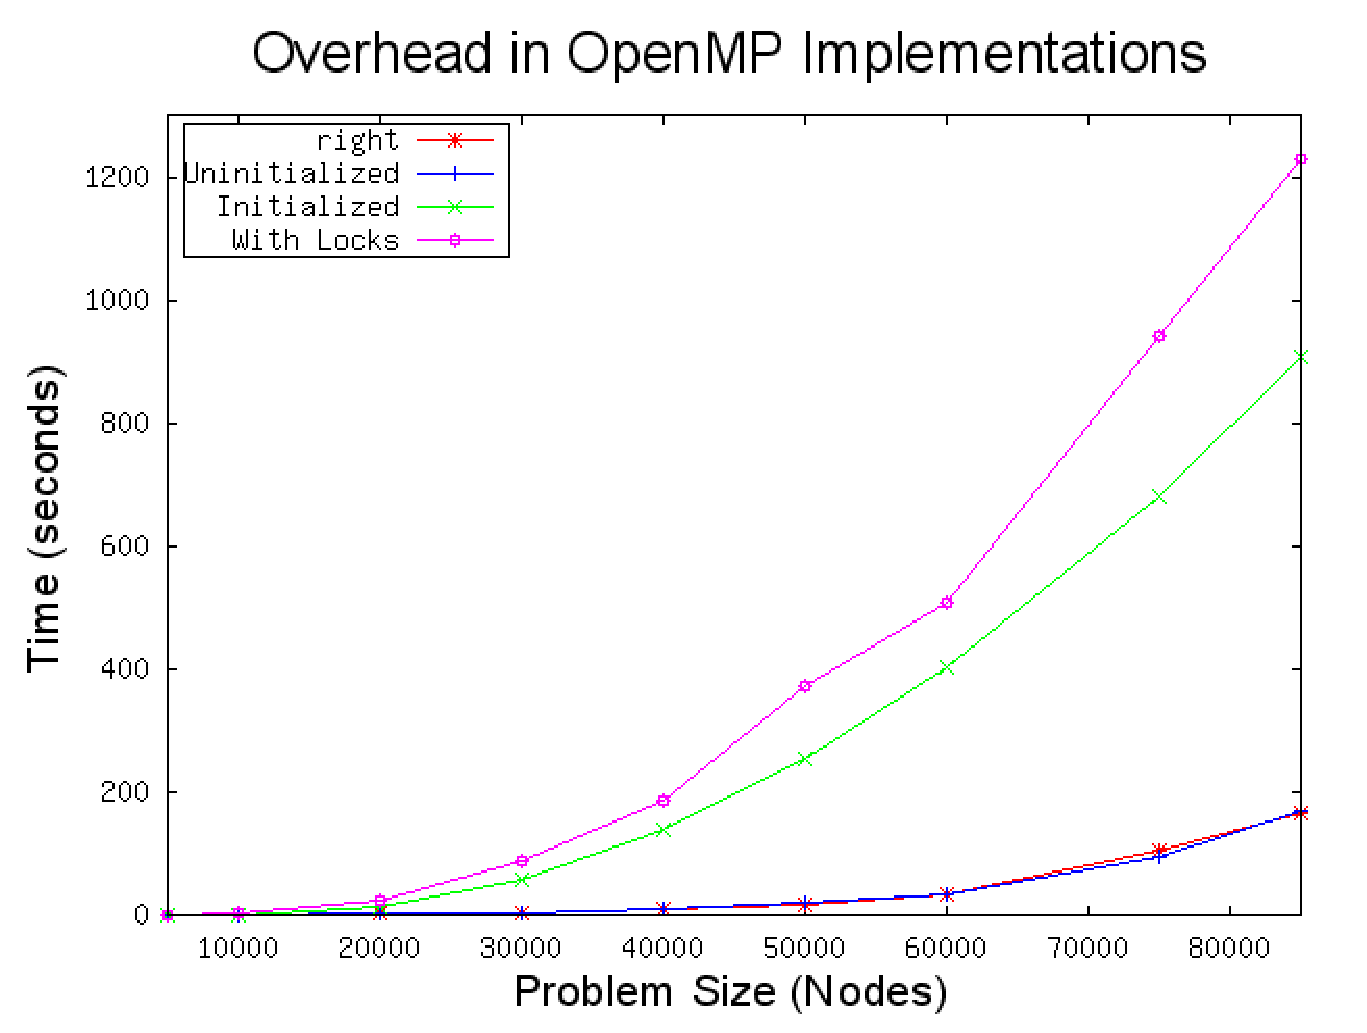
\includegraphics[width=0.75\textwidth]{images/figura1.eps}
\caption{Ejemplo de figura}
\label{fig:1}
\end{center}
\end{figure}
%------------------------------------------------------------------------------


%------------------------------------------------------------------------------
%--------------------------------------------------------------------------
\begin{table}[!ht]
\begin{center}
\begin{tabular}{|c|c|} \hline 
\textbf{Tiempo  } & \textbf{Velocidad} \\ 
\textbf{($\pm$ 0.001 s)} & \textbf{($\pm$ 0.1 m/s)} \\ \hline \hline
1.234 &
67.8
\\
\hline

2.345 &
78.9
\\
\hline

3.456 &
89.1
\\
\hline

4.567 &
91.2
\\
\hline

\end{tabular}
\end{center}
\caption{Resultados experimentales de tiempo (s) y velocidad (m/s)}
\label{tab:1}
\end{table}


%------------------------------------------------------------------------------

%++++++++++++++++++++++++++++++++++++++++++++++++++++++++++++++++++++++++++++++
\section{An�lisis de los resultados}
\label{3:sec:4}

bla, bla, etc. 



%%%%%%%%%%%%%%%%%%%%%%%%%%%%%%%%%%%%%%%%%%%%%%%%%%%%%%%%%%%%%%%%%%%%%%%%%%%%%%%
\chapter{Conclusiones}
\label{chapter:conclusiones}

%%%%%%%%%%%%%%%%%%%%%%%%%%%%%%%%%%%%%%%%%%%%%%%%%%%%%%%%%%%%%%%%%%%%%%%%%%%%%
% Chapter 4: Conclusiones y Trabajos Futuros 
%%%%%%%%%%%%%%%%%%%%%%%%%%%%%%%%%%%%%%%%%%%%%%%%%%%%%%%%%%%%%%%%%%%%%%%%%%%%%%%

bla, bla, bla, etc.


%%%%%%%%%%%%%%%%%%%%%%%%%%%%%%%%%%%%%%%%%%%%%%%%%%%%%%%%%%%%%%%%%%%%%%%%%%%%%%%

%%%%%%%%%%%%%%%%%%%%%%%%%%%%%%%%%%%%%%%%%%%%%%%%%%%%%%%%%%%%%%%%%%%%%%%%%%%%%%%
\newpage{\pagestyle{empty}\cleardoublepage}
\thispagestyle{empty}
\begin{appendix}

\chapter{T�tulo del Ap�ndice 1}
\label{appendix:1}

\section{Algoritmo XXX}
\label{Apendice1:XXX}

\begin{center}
\begin{footnotesize}
\begin{verbatim}
###################################################################################
# Fichero .py
###################################################################################
#
# AUTORES
#   
# FECHA
#
# DESCRIPCION
#
###################################################################################
\end{verbatim}
\end{footnotesize}
\end{center}

\section{Algoritmo YYY}
\label{Apendice1:YYY}

\begin{center}
\begin{footnotesize}
\begin{verbatim}
/###################################################################################
 # Fichero .h
 ###################################################################################
 #
 # AUTORES
 #
 # FECHA
 #
 # DESCRIPCION
 #
 ##################################################################################
\end{verbatim}
\end{footnotesize}
\end{center}


\chapter{T�tulo del Ap�ndice 2}
\label{appendix:2}

\section{Otro apendice: Seccion 1}
\label{Apendice2:label}

\begin{center}
\begin{footnotesize}

\begin{verbatim}
Texto
\end{verbatim}

\end{footnotesize}
\end{center}

\section{Otro apendice: Seccion 2}
\label{Apendice2:label2}

\begin{center}
\begin{footnotesize}

\begin{verbatim}
Texto
\end{verbatim}


\end{footnotesize}
\end{center}


\end{appendix}

%%%%%%%%%%%%%%%%%%%%%%%%%%%%%%%%%%%%%%%%%%%%%%%%%%%%%%%%%%%%%%%%%%%%%%%%%%%%%%%
\addcontentsline{toc}{chapter}{Bibliograf�a}
\bibliographystyle{plain}


\bibliography{bib/references}
\nocite{*}

%%%%%%%%%%%%%%%%%%%%%%%%%%%%%%%%%%%%%%%%%%%%%%%%%%%%%%%%%%%%%%%%%%%%%%%%%%%%%%%

\end{document}
